\documentclass[a4paper,titlepage]{article}
\usepackage[utf8]{inputenc}
\usepackage[spanish]{babel}
\date{\today}
\pagestyle{empty}
\usepackage{natbib}
\usepackage{graphicx}
\usepackage{tikz,pgfplots}
\usetikzlibrary{pgfplots.statistics}
\usepackage{subcaption}
\usepackage[hidelinks]{hyperref}
\usepackage[a4paper,margin=3cm]{geometry}
\spanishdecimal{.}
\usepackage{tikz-3dplot}
\spanishdecimal{.}
\pgfplotsset{compat=1.5}
\usepackage{multirow}
\usepackage{steinmetz}

%%%%%%%% Matematicas
\usepackage{amsmath}
\usepackage{amsfonts}
\usepackage{amssymb}
\usepackage{booktabs}


\title{Práctica n$^{\circ}$7: Obtención Curvas Magnéticas en C.A.\\
\small Laboratorio de Instrumentación Eléctrica\\
\small4$^{\circ}$B, I.E.M}
\author{Gonzalo Sánchez Contreras\\
Antonio Rubí Rodríguez\\
Ignacio Sanz Soriano
}
\date{22 de noviembre de 2016}

\usepackage{natbib}
\usepackage{graphicx}
\usepackage[cuteinductors]{circuitikz}
\usepackage{fancyhdr}
\renewcommand{\headrulewidth}{0.0pt}
\fancyhead[R]{\textit{4$^{\circ}$B, I.E.M.}}\fancyhead[L]{\empty}
\fancyfoot[R]{\textit{Laboratorio de Instrumentación Eléctrica}}\fancyfoot[L]{\textit{Grupo 4}}\fancyfoot[C]{\empty}
\pagestyle{fancy}
\begin{document}

\maketitle
\newpage{\ } 
\thispagestyle{empty}
\newpage
\section*{Ensayo 7.1. Características dinámicas B-H y S-B del material ferromagnético }
\noindent\textbf{\underline{Enunciado}}: Obtención de las características dinámicas B-H y S-B de un material ferromagnético .\\   

\noindent\textbf{\underline{Esquema}}:

\begin{center}
    \begin{tikzpicture}[american voltages] 
        \draw (0,0) to [isourcesin] (0,2)
        to [short] (1,2);
        \draw[thick] (1.75,1) circle (0.4cm);
        \draw[thick] (2.25,1) circle (0.4cm);
        \draw [<-,thick] (2.5,1.5)--(1.5,0.5);
        \draw (0,0) to [short,-] (1,0)
        to [short] (1.4671,0.7171)
        (1,2) to [short] (1.4671,1.2828)
        (2.53284,1.2828) to [short] (3,2)
        (2.53284,0.7171) to [short] (3,0)
        (3,2) to [short,-] (5.258,2)
        % (3,0) to [short,-] (5.258,0)
        (3,0) to [R,l^=$R_1$] (5.258,0)
        
        %Parte derecha
        (6.742,2) to [short,-] (7.5,2)
        to [R,l^=$R_2$,-] (9.5,2)
        to [-] (10,2)
        to [capacitor,l_=$C$] (10,0)
        to [short,-] (6.742,0)
        ;
        
        % OSCILOSCOPIO
        \draw (11,2) to [short,-] (11,-1.625)
        to [-] (13,-1.625)
        to [-] (13,2)
        to [-]  (11,2); 
        
        % Chanel II
        \draw (10,1.5) to [short,*-] (10.75,1.5)
        to [-] (10.75,1.125)
        to [short,-o] (11,1.125)
        (10,0.5) to [short,*-] (10.75,0.5)
        to [-] (10.75,0.875)
        to [short,-o] (11,0.875)
        to [-] (11.25,0.875)
        to [-] (11.25,0.75)
        (11.25,0.875) to [-]  (11.25,1);
        
        % Chanel I
        \draw (3.25,0) to [short,*-] (3.25,-1.25)
        (5,0) to [short,*-] (5,-1)
        (5,-1) to [short,-] (7.85,-1)
        to [short,-] (7.85,-0.5)
        to [short,-o] (11,-0.5)
        (3.25,-1.25) to [short,-] (8.1,-1.25)
        to [short,-] (8.1,-0.75)
        to [short,-o] (11,-0.75) 
        to [-] (11.25,-0.75)
        to [-] (11.25,-0.875)
        (11.25,-0.75) to [-]  (11.25,-0.625);
        
        % Detalles 
        \draw[] (5.425,2.15) node[left]{\small$\bullet$};
        \draw[] (6.6,2.15) node[right]{\small$\bullet$};
        \draw[] (11.25,1) node[right]{\small CHII};
        \draw[] (11.25,-0.625) node[right]{\small CHI};
        \draw[] (12.5,0.1875) node[rotate=90]{OSCILOSCOPIO};
        % Circulo exterior
        \draw[thick,dashed] (6,1) circle (1.25cm);
        
        % Cuadro interior
        \draw[thick,dashed] (6,1) circle (1.15cm);
        \draw[thick,dashed] (6,1) circle (1.05cm);
        
        % Voltímetros
        \draw[thick] (7.85,1) circle (0.35cm);
        \draw[] (7.85,1) node[]{V$_2$};
        \draw (7.85,2) to [short,*-] (7.85,1.35);
        \draw[] (7.85,0) to [short,*-] (7.85,0.65);
        \draw[thick,dashed] (6,1) circle (1.05cm);
        
        \draw[thick] (4.125,-0.65) circle (0.35cm);
        \draw[] (4.125,-0.65) node[]{V$_1$};
        \draw (3.25,-0.65) to [short,*-] (3.775,-0.65);
        \draw[] (4.475,-0.65) to [short,-*] (5,-0.65);
        
        % Arrolamientos izquierda abajo
        \draw[] (4.85,1) ellipse (0.25cm and 0.075cm);
        %\draw[thin] (5.851,0.95) ellipse (0.25cm and 0.05cm);
        \draw[] (4.8544,0.899) ellipse (0.25cm and 0.075cm);
        %\draw[thin] (5.859,0.849) ellipse (0.25cm and 0.05cm);
        \draw[] (4.867,0.800) ellipse (0.25cm and 0.075cm);
        %\draw[thin] (5.889,0.751) ellipse (0.25cm and 0.05cm);
        \draw[] (4.889,0.702) ellipse (0.25cm and 0.075cm);
        \draw[] (4.919,0.606) ellipse (0.25cm and 0.075cm);
        \draw[] (4.957,0.514) ellipse (0.25cm and 0.075cm);
        \draw[] (5.004,0.425) ellipse (0.25cm and 0.075cm);
        \draw[] (5.06,0.34) ellipse (0.25cm and 0.075cm);
        \draw[] (5.12,0.261) ellipse (0.25cm and 0.075cm);
        \draw[] (5.186,0.187) ellipse (0.25cm and 0.075cm);
        \draw[] (5.260,0.119) ellipse (0.25cm and 0.075cm);
        \draw[] (5.340,0.058) ellipse (0.25cm and 0.075cm);
        % \draw[thick] (6.425,0.004) ellipse (0.25cm and 0.075cm);
        
        % Arrolamientos izquierda arriba
        %\draw[thin] (5.851,0.95) ellipse (0.25cm and 0.05cm);
        \draw[] (4.8544,1.10) ellipse (0.25cm and 0.075cm);
        %\draw[thin] (5.859,0.849) ellipse (0.25cm and 0.05cm);
        \draw[] (4.867,1.199) ellipse (0.25cm and 0.075cm);
        %\draw[thin] (5.889,0.751) ellipse (0.25cm and 0.05cm);
        \draw[] (4.889,1.297) ellipse (0.25cm and 0.075cm);
        \draw[] (4.919,1.393) ellipse (0.25cm and 0.075cm);
        \draw[] (4.957,1.486) ellipse (0.25cm and 0.075cm);
        \draw[] (5.004,1.575) ellipse (0.25cm and 0.075cm);
        \draw[] (5.06,1.659) ellipse (0.25cm and 0.075cm);
        \draw[] (5.12,1.7392) ellipse (0.25cm and 0.075cm);
        \draw[] (5.186,1.813) ellipse (0.25cm and 0.075cm);
        \draw[] (5.260,1.881) ellipse (0.25cm and 0.075cm);
        \draw[] (5.340,1.942) ellipse (0.25cm and 0.075cm);
        
        
        % Arrolamientos derecha arriba
        \draw[] (7.15,1) ellipse (0.25cm and 0.075cm);
        %\draw[thin] (5.851,0.95) ellipse (0.25cm and 0.05cm);
        \draw[] (7.145,1.10) ellipse (0.25cm and 0.075cm);
        %\draw[thin] (5.859,0.849) ellipse (0.25cm and 0.05cm);
        \draw[] (7.132,1.199) ellipse (0.25cm and 0.075cm);
        %\draw[thin] (5.889,0.751) ellipse (0.25cm and 0.05cm);
        \draw[] (7.111,1.297) ellipse (0.25cm and 0.075cm);
        \draw[] (7.081,1.393) ellipse (0.25cm and 0.075cm);
        \draw[] (7.042,1.486) ellipse (0.25cm and 0.075cm);
        \draw[] (6.996,1.575) ellipse (0.25cm and 0.075cm);
        \draw[] (6.942,1.659) ellipse (0.25cm and 0.075cm);
        \draw[] (6.881,1.7392) ellipse (0.25cm and 0.075cm);
        \draw[] (6.8132,1.813) ellipse (0.25cm and 0.075cm);
        \draw[] (6.739,1.881) ellipse (0.25cm and 0.075cm);
        \draw[] (6.659,1.942) ellipse (0.25cm and 0.075cm);
        
        
        % Arrolamientos derecha abajo
        % \draw[] (7.15,1) ellipse (0.25cm and 0.075cm);
        %\draw[thin] (5.851,0.95) ellipse (0.25cm and 0.05cm);
        \draw[] (7.145,0.899) ellipse (0.25cm and 0.075cm);
        %\draw[thin] (5.859,0.849) ellipse (0.25cm and 0.05cm);
        \draw[] (7.132,0.800) ellipse (0.25cm and 0.075cm);
        %\draw[thin] (5.889,0.751) ellipse (0.25cm and 0.05cm);
        \draw[] (7.111,0.702) ellipse (0.25cm and 0.075cm);
        \draw[] (7.080,0.606) ellipse (0.25cm and 0.075cm);
        \draw[] (7.042,0.514) ellipse (0.25cm and 0.075cm);
        \draw[] (6.995,0.425) ellipse (0.25cm and 0.075cm);
        \draw[] (6.942,0.34) ellipse (0.25cm and 0.075cm);
        \draw[] (6.881,0.261) ellipse (0.25cm and 0.075cm);
        \draw[] (6.813,0.187) ellipse (0.25cm and 0.075cm);
        \draw[] (6.739,0.119) ellipse (0.25cm and 0.075cm);
        \draw[] (6.659,0.058) ellipse (0.25cm and 0.075cm);
    \end{tikzpicture}
\end{center}

\noindent\textbf{\underline{Preparación}}: Todos los aparatos serán seleccionados para medir con la mejor precisión posible un campo B de cresta ($\hat{B}$) de 1.5 T. Las características del anillo de Rowland a ensayar son:
\begin{itemize}
    \item Devanado interior: $N_{int}=329$ espiras; 0.9 $\Omega$; $I_{max}=1$ A.
    \item Devanado exterior: $N_{ext}=68$ espiras; 60 m$\Omega$; $I_{max}=5$ A.
    \item Sección neta: 0.92 cm$^2$, longitud media $l=34$ cm.
    \item Densidad $\rho=7650$ kg/m$^3$.
    \item Valores aproximados para $\hat{B}=1.5$ T: $H_{ef}\approx30$ A/m, $\hat{H}\approx50$ A/m.
\end{itemize}
La tensión en el arrollamiento exterior o de excitación ($N_{exc} = 68$ espiras) para un campo $\hat{B}$ de 1.5 T es :
\begin{gather*}
    U_{exc}=4.44\cdot N_{exc}\cdot f\cdot \hat{B}\cdot S=4.44\cdot 68\cdot50\cdot1.5\cdot0.92\cdot10^{-4}= 2.083\:V
\end{gather*}
Aplicando la relación de transformación del anillo a la tensión del arrollamiento de excitación, la tensión inducida en el arrollamiento  interior ($N_{int} = 329$ espiras) es :
\begin{gather*}
    U_{ind}=U_{exc}\cdot\frac{N_{int}}{N_{ext}}=2.083\cdot\frac{329}{68}=10.08\:V
\end{gather*}

\textbf{\textit{Selección de la resistencia $\mathbf{R_1}$}}. Se busca una resistencia $R_1$ lo más pequeña posible para que la tensión de excitación ($U_{exc}$) no se vea afectada y se mantenga sinusoidal. Se elegirá la resistencia \textit{shunt} de 100 m$\Omega$, 1.5 A, 1\%, por ser la más pequeña de entre las disponibles, presentar una buena precisión en comparación con las restantes (1\%) y aguantar sin problemas la intensidad del ensayo, ya la intensidad máxima que soporta es de 1.5 A, y la intensidad prevista en el ensayo es de 150 mA, para un campo $\hat{B}$ de 1.5 T. La tensión que caerá en la resistencia será, por tanto:
\begin{gather*}
    I_{exc}=\frac{H_{ef}\cdot l}{N_{exc}}=\frac{30\cdot0.34}{68}=150\:mA\\
    U_{R_1} = I_{exc}\cdot R_1 = 0.15\cdot0.1=15\:mV
\end{gather*}
Se comprueba que efectivamente la tensión de excitación ($U_{exc}$) es mucho mayor ($n$ veces) que la tensión en la resistencia $R_1$:
\begin{gather*}
    n=\frac{U_{exc}}{U_{R_1}}= \frac{2.083}{0.015}= 138.9\\
    R_1\cdot I_{exc}\ll U_{exc}
\end{gather*}
por lo que será esta  resistencia de 100 m$\Omega$, 1.5 A, 1\% la que se utilizará en el ensayo.
\newpage
\textbf{\textit{Selección de la resistencia $\mathbf{R_2}$}}. Se escogerá una resistencia de tal forma que se cumplan las condiciones necesarias para el ensayo, a saber, que el anillo esté en vacío y que se pueda aproximar la intensidad inducida ($i_{ind}$) como $\dfrac{u_{ind}}{R_2}$ en el condensador. 

Para poder asumir que el anillo de Rowland está en vacío, se ha de cumplir que la intensidad inducida es como mucho el 1\% de la intensidad de magnetización (estimada en 150 mA). Escogemos por ello como resistencia $R_2$, la de 100 k$\Omega$ de la caja de décadas, clase 0.1, 0.25 W, por satisfacer estos tres requisitos:  buena precisión, capacidad de disipar la potencia del ensayo y con una intensidad circulando por ella de valor:
\begin{gather*}
    I_{ind} = \frac{U_{ind}}{R_2}= \frac{10.08}{100\cdot10^3}=0.1\:mA
\end{gather*}
Sabiendo, que la intensidad máxima en el arrollamiento de excitación es de 1.5 mA, en el ensayo con $R_2$ se tiene que:
\begin{gather*}
    I_{ind}^{exc}= I_{ind}\cdot\frac{N_{exc}}{N_{int}}=0.1\cdot\frac{68}{329}= 0.021\:mA
\end{gather*}
Se puede asumir que efectivamente el anillo esta trabajando en vacío, pues $0.021\ll1.5$ mA, así que será la resistencia de 100 k$\Omega$ la que se empleará en el ensayo.\\

\textbf{\textit{Selección del condensador $\mathbf{C}$}}. A continuación, se ha de seleccionar el condensador de forma que la impedancia del mismo ($Z_C$) sea al menos cincuenta veces menor que la de $R_2$. De esta forma, se podrán escoger los condensadores que cumplan que:
\begin{gather*}
    R_2 \geq 50\cdot\frac{1}{\omega\cdot C}
\end{gather*}
\begin{gather*}
    C \geq 50\cdot\frac{1}{R_2\cdot \omega}=50\cdot\frac{1}{100\cdot10^3\cdot100\pi}=1.592\:\mu F
\end{gather*}
\begin{gather*}
    C\geq1.592\:\mu F
\end{gather*}
Entre las distintas opciones, se encuentran condensadores de distintas capacidades: $2\mu F$, $5\mu F$, $10\mu F$, $20\mu F$, $50\mu F$, 250 V, clase 5. Ya que todos satisfacen ambas condiciones, se elegirá aquel en el que tenga una tensión tal, que permita medir con la máxima precisión posible en el osciloscopio, por lo que se escogerá junto con los alcances en el osciloscopio a continuación.\\

\textbf{\textit{Selección de la alimentación}}. Para seleccionar la alimentación más adecuada para el ensayo, ha de considerarse que tiene que proporcionar la mejor resolución posible. Se dispone de la red de 220 V del laboratorio y de una fuente de 100 V, 50 Hz. Como se tiene una tensión de excitación ($U_{exc}$) de 2.08 V, se selecciona el VARIAC de 220/0-6 V, 15 A, resolución de 20 mV para 220 V a la entrada frente al VARIAC de 220/0-250, 4 A, resolución de 1 V para 220 V a la entrada, pues el primero proporciona la tensión necesaria para el ensayo y además presenta mejor resolución, por lo que será esté último el VARIAC a emplear en el ensayo. También se calculará la

Se calculan las resoluciones obtenidas para cada una de las fuentes de alimentación disponibles. Así, se tiene que:
\begin{itemize}
    \item Red de 220 V. Alimentando el VARIAC 220/0-6 V, entre fase y neutro, 127 V se tiene una resolución de:
    \begin{gather*}
        \Delta U_{ind} = \Delta U\cdot \frac{127}{220}\cdot\frac{N_{int}}{N_{ext}} = 20\cdot\frac{127}{220}\cdot\frac{329}{68}= 55.86\:mV 
    \end{gather*}
    \item Fuente de 100 V. Alimentando el VARIAC 220/0-6 V se tiene una resolución de:
    \begin{gather*}
        \Delta U_{ind} = \Delta U\cdot \frac{100}{220}\cdot\frac{N_{int}}{N_{ext}} = 20\cdot\frac{100}{220}\cdot\frac{329}{68}= 43.98\:mV 
    \end{gather*}
\end{itemize}
Se observa que la resolución en el lado de la tensión de inducido ($\Delta U_{ind}$) es mejor con la fuente de 100 V que alimentando con la red entre fase y neutro, 127 V, por lo que se escoge como alimentación la fuente de 100 V, 50 Hz, que proporciona los 2.08 V necesarios para el ensayo, y se empleará el VARIAC 220/0-6 V, 15 A, resolución de 20 mV para 220 V a la entrada.
\newpage
\textbf{\textit{Selección de los voltímetros}}. Los voltímetros se elegirán de manera que se mida con la mejor precisión posible la tensión en la resistencia $R_1$ y la tensión de inducido $U_{ind}$. Para seleccionar los voltímetros se ha de tener en cuenta el tipo de tensión que se va a medir (sinusoidal o no sinusoidal). Para las dos tensiones a medir $U_{R_1}$ y $U_{ind}$, se tiene que:
\begin{itemize}
    \item Tensión $U_{R_1}$. Se espera una tensión no sinusoidal, debido a  que la intensidad de excitación tampoco lo es, por lo que se utilizará el Multímetro digital PROMAX PD-183 (20000 cuentas, verdadero valor eficaz), en alcance de 200 mV. La incertidumbre esperada en la medida es:
    \begin{gather*}
        \alpha(U_{R_1})=\frac{1}{100}\cdot U_{R_1}+10\cdot0.01=\frac{0.8}{100}\cdot 15+3\cdot0.01=0.25\:mV\\
        \varepsilon(U_{R_1})=\frac{\alpha(U_{R_1})}{U_{R_1}}\cdot100=\frac{0.25}{15}\cdot100=1.67\%
    \end{gather*}
    \item Tensión $U_{ind}$. Se espera una tensión sinusoidal, debido a  que la tensión de excitación también lo es, por lo que se utilizará el polímetro digital PROMAX FP–2b (2000 cuentas), en alcance de 20 V . La incertidumbre esperada en la medida es:
    \begin{gather*}
        \alpha(U_{ind})=\frac{0.8}{100}\cdot U_{ind}+3\cdot0.01=\frac{0.8}{100}\cdot 10.08+3\cdot0.01=0.0.11\:V\\
        \varepsilon(U_{ind})=\frac{\alpha(U_{ind})}{U_{ind}}\cdot100=\frac{0.11}{10.08}\cdot100=1.1\%
    \end{gather*}
\end{itemize}

\textbf{\textit{Selección de los alcances del osciloscopio}}. Los alcances del osciloscopio se ajustarán de tal forma que se mida con la mejor precisión posible la tensión de pico en la resistencia $R_1$ y en el condensador $C$.\\ 

\textbf{Eje de tiempos}. Por tratarse de ondas de frecuencia igual a 50 Hz, se necesitará un alcance de tiempos de 2 ms/div, y escogiendo el alcance inmediatamente superior se tienen 2.5 ms/div en el eje horizontal del osciloscopio.\\

\textbf{Canal I (CHI)}. Para una tensión en la resistencia $R_1$ de 15 mV, se tiene una tensión pico- pico de:
\begin{gather*}
    U_{{R_{1}}_{p-p}}= U_{R_1}\cdot R_1\cdot2\cdot\sqrt{2}= 42.42\:mV
\end{gather*}
por lo que se necesitan como mínimo en el osciloscopio para 8 divisiones en el eje vertical:
\begin{gather*}
    \frac{U_{{R_{1}}_{p-p}}}{8\:div}=5.30\:mV/div
\end{gather*}
y seleccionado el alcance inmediatamente superior se consigue un alcance de \textbf{10 mV/div} para el canal I.\\

\textbf{Canal II (CHII)}. Como se dispone de varios condensadores, de la misma precisión (5\%), se seleccionará aquel que tenga una caída de tensión que sea lo más cercana posible su respectivo alcance inmediatamente superior en el osciloscopio. Para ello, se calcula la tensión en el condensador como:
\begin{gather*}
    U_C=U_{ind}\cdot\frac{\frac{1}{j\omega\cdot C}}{R_2+\frac{1}{j\omega\cdot C}}=10.08\cdot\frac{\frac{1}{j100\pi\cdot C}}{100\cdot10^3+\frac{1}{j100\pi\cdot C}}
\end{gather*}
donde C son las distintas capacidades disponibles.
Para cada capacidad ($C$) se han obtenido las tensiones eficaces, pico-pico y en mV/div para poder seleccionar el mejor alcance en el osciloscopio. En la tabla se presentan todas las combinaciones posibles:
\newpage
% \setlength{\extrarowheight}{4.5pt}
{\setlength{\arrayrulewidth}{0.75pt}
\begin{table}[htbp]
    \centering
    \begin{tabular}[t]{c|c|c|c|c}
        \textbf{C} \small\textbf{($\mathbf{\mu}$F)}& $\mathbf{U_C}$ \small\textbf{(mV)}& $\mathbf{U_{C_{p-p}}}$ \small\textbf{(mV)} & $\mathbf{U_C}$ \small\textbf{(mV/div)}& \small\textbf{Alcance Osc.}\\
        \hline
        $50$  &  6.4  &  18.1  &  2.26  & 5 \\
        \hline
        $20$  &  16  & 45.25   &  5.65  & 10 \\
        \hline
        $10$  &  32  &  90.79  &  11.35  & 20 \\
        \hline
        $5$  &  64.2  &  181.6  &  22.7  & 50 \\
            \hline
        $2$  &  160.4  &  453.7  &  56.71  & 100 \\
    \end{tabular}
\end{table} 

\noindent Los condensadores de 10 $\mu F$ y de 2 $\mu F$ presentan la misma precisión para sus respectivos alcances en el osciloscopio. Se escoge el condensador de capacidad $C=10$ $\mu F$, clase 5, 250 V, por ser el proporciona una tensión de pico lo más próxima al alcance inmediatamente superior, por lo que será la tensión que se mida con mejor precisión de entre todas las posibles.
Además, se escogerá un alcance de \textbf{20 mV/div} en el eje vertical del osciloscopio en el canal II.\\

\noindent\textbf{\underline{Lista de Aparatos}}:\\

\noindent Aparatos de Precisión:
\begin{itemize}
    \item V1: Multímetro digital PROMAX PD-183 (20000 cuentas, verdadero valor eficaz). Como voltímetro: \underline{200} mV, 2, 20, 200, 1000 V. Resistencia interna: 10M$\Omega$. Precisión: 1\%lect. + 10díg. en CA.
    \item V2: Polímetro digital PROMAX FP–2b (2000 cuentas). Como voltímetro: 200 mV, 2, \underline{20}, 200, 1000 V. Resistencia interna: 10M$\Omega$. Precisión: 0.8\%lect. + 3díg. en CA.
    \item Osciloscopio: 
    Alcances tiempo:(1–2.5–5–10–25–50–100–250–500)$\mu$s/div\\(1–\underline{2.5}–5–10–25–50–100–250–500)ms/div.\\
    CHI: Alcances tensión: (5–\underline{10}–20–50–100–200–500)mV/div–(1–2–5)V/div.\\
    CHII: Alcances tensión: (5–10-\underline{20}–50–100–200–500)mV/div–(1–2–5)V/div.\\
    Eje horizontal: 10div; precisión: 2\% en modo XT; 3\% en modo XY.\\
    Eje vertical: 8div; precisión: 2\%. 
    \item $R_1$: Resistencia (shunt): 100m$\Omega$, 1.5A; 1\%.
    \item $R_2$: Caja de resistencias 2x(0.1, 1, 10 y \underline{100})k$\Omega$ clase 0.1, 0.25W.
    \item $C$: Caja de condensadores de 100nF, 470nF, 2 $\mu$F, \underline{10} $\mu$F, 50 $\mu$F; clase 5; 250V. 
\end{itemize}

\noindent Aparatos de Auxiliares:
\begin{itemize}
    \item Autotransformador VARIAC 220V/0–6V (con aislamiento galvánico); 15A; resolución para entrada 220V: 20mV.
    \item Fuente de tensión 100 V, 50 Hz. 
\end{itemize}

\noindent\textbf{\underline{Medidas}}:
{\setlength{\arrayrulewidth}{1pt}
\begin{table}[h!]
    \flushleft
    \begin{tabular}[t]{|c|c|c|c|c|c|c|c|c|c|c|c|}
        \hline
        \multicolumn{12}{|c|}{\textbf{Ensayo a 50 Hz}} \\
        \cline{1-12}
        \multirow{2}{1.5cm}{\textbf{Objetivo}}& $B$ (T) & 0.4 & 0.5 & 0.6 & 0.8 & 0.9 & 1.0 & 1.1 & 1.2 & 1.4&1.5\\
        \cline{2-12}
        &$U_B$ (V) &0.56 &0.69&0.83 & 1.11&1.25 &1.39 &1.53 &1.67 &1.94 &2.08 \\
        \hline
    \end{tabular}
\end{table}
\begin{table}[h!]
    \centering
    \begin{tabular}[t]{|c|c|c|c|c|c|c|c|c|c|c|c|c|}
        \hline
        \multirow{4}{1.5cm}{\textbf{Medidas}}& $\mathbf{U_H}$ (mV) &3.58& 4.9&5.62& 6.01&6.59 & 7.18& 7.78 & 8.45& 10.22&11.84 \\
        \cline{2-12}
        &$\mathbf{U_B}$ (V) &2.68 &3.35 &4.04 &5.40  &6.06 &6.76 & 7.42& 8.09&  9.42& 10.09\\
        \cline{2-12}
        &$\mathbf{U_{CHI_{,cresta}}}$ (mV) &7 &8 &8.9 & 9.8 & 10.5& 11.6&11.7 &12.1 &  13.2& 17.2 \\
        \cline{2-12}
        &$\mathbf{U_{CHII_{,cresta}}}$ (mV) &70 &79 &96 &125 & 140& 155 &170 &185 &  220&232\\
        \cline{1-12}
    \end{tabular}
\end{table}
\begin{table}[h!]
    \flushleft
    \begin{tabular}[l]{|l|l|c|c|c|c|c|c|c|c|c|c|}
        \hline
        \multirow{4}{1.5cm}{\small\textbf{Cálculo a partir de medidas}}&\small $\mathbf{B_{cresta}}$ $\mathbf{U_B}$\textbf{(T)}&0.39 &0.49 &0.60 &0.80 &0.90 &1.00 & 1.10&1.20 &1.40 &1.50 \\
        \cline{2-12}
        &\small$\mathbf{B_{cresta}}$ $\mathbf{U_{CHII}}$ \textbf{(T)} &0.462 &0.52 &0.63 &0.82 &0.92 &1.024 &1.12 & 1.22&1.45 &1.53 \\
        \cline{2-12}
        &\small$\mathbf{H_{eficaz}}$ $\mathbf{U_{H}}$\textbf{(A/m)}  &7.16 &9.8 &11.24 &12.02 &13.18 &14.36 &15.56 &16.9 &20.44 &23.68 \\
        \cline{2-12}
        &\small$\mathbf{H_{cresta}}$ $\mathbf{U_{CHI}}$ \textbf{(A/m)}& 14& 16&17.8 &19.6 &21 &23.2 &23.4 &24.2 &26.4 &34.4\\
        \cline{2-12}
        &\small$\mathbf{S_{esp}}$ \textbf{(VA/kg)}& 0.08& 0.14&0.2 &0.28 &0.34 &0.42 &0.50 &0.59 &0.83 &1.03\\
        \cline{1-12}
    \end{tabular}
\end{table}
\newpage
\noindent\textbf{\underline{Resultados}}:\\

\textbf{1. $\mathbf{B_{cresta}}$ (T)-$\mathbf{H_{ef}}$ (A/m) y $\mathbf{B_{cresta}}$ (T)-$\mathbf{H_{cresta}}$ (A/m)}\\
\begin{figure}[ht]
 \centering
     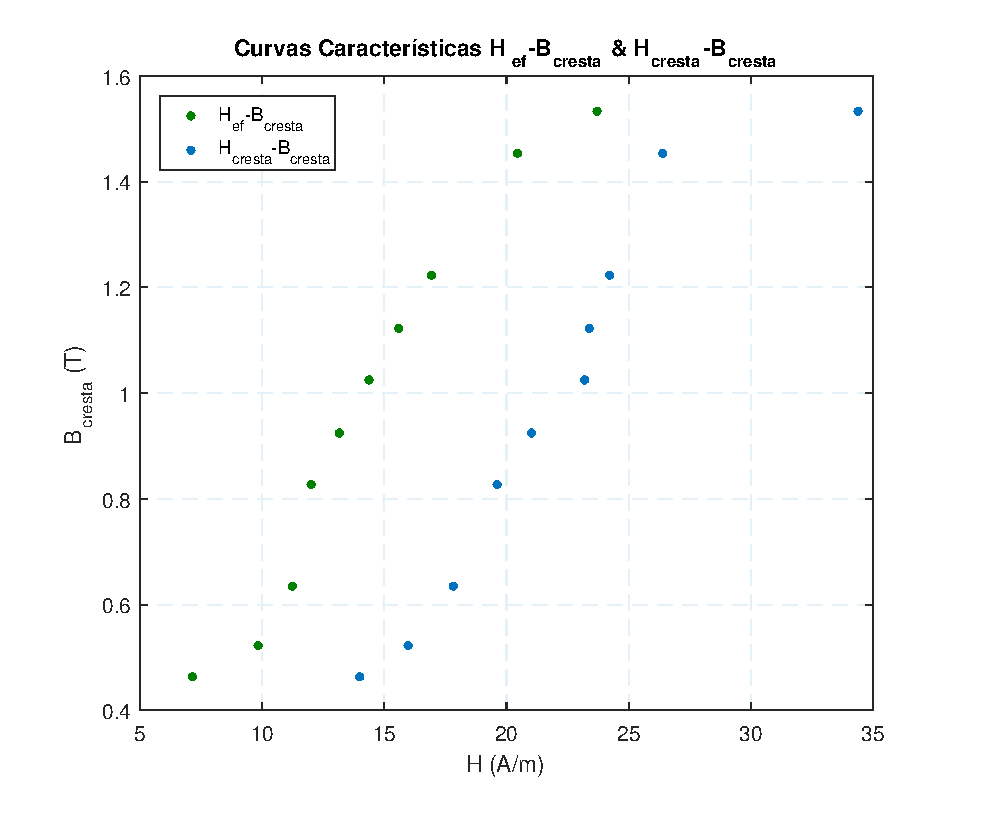
\includegraphics[width=\textwidth]{byh.eps}
\end{figure}
\newpage
\textbf{2. $\mathbf{S_{esp}}$ (VA/kg)-$\mathbf{B_{cresta}}$ (T)}\\
\begin{figure}[ht]
 \centering
     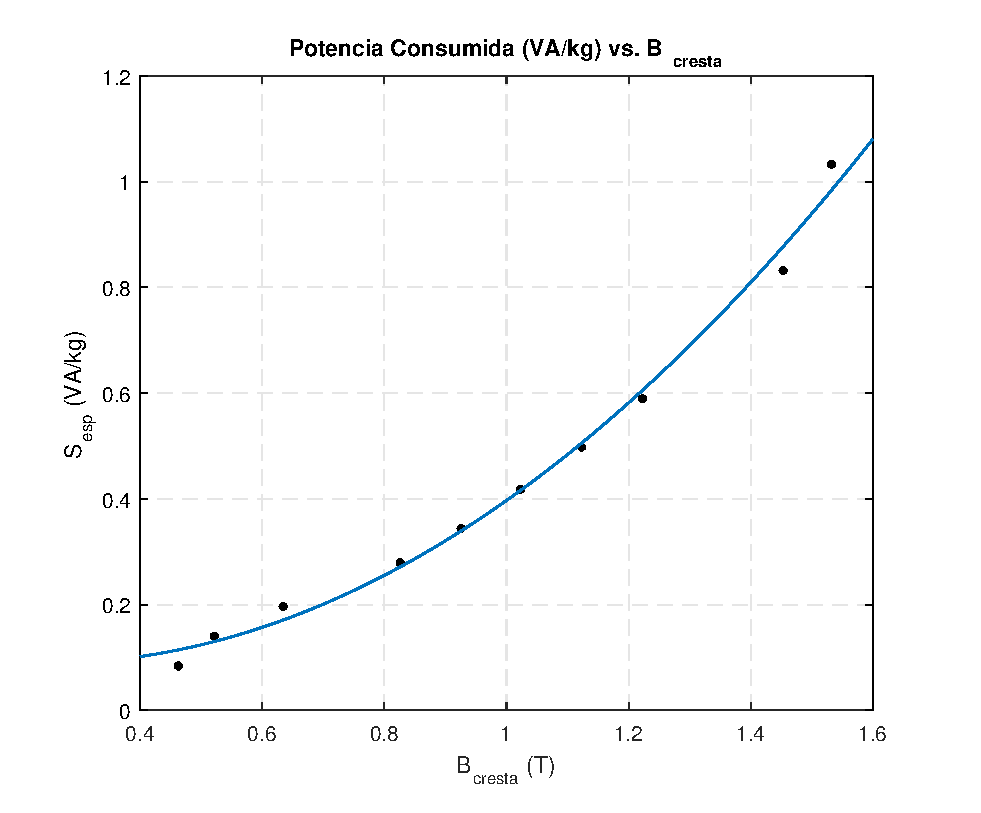
\includegraphics[width=\textwidth]{potencia.eps}
\end{figure}

\noindent\textbf{\underline{Conclusiones}}:
El ensayo se ha realizado a 0.1 $\Omega$ cuando debería ser a 1 $\Omega$. Esto se debe a que se ha priorizado el no afectar a la forma de la tensión sinusoidal. Sin embargo, a pesar de que si el ensayo se realiza con una $R_1=1$ $\Omega$, (obteniéndose una $U_{r1}$ que es apenas 13 veces menor a la $U_{exc}$) el valor de $U_{ind}$ medido por el voltímetro $V_2$ (\textit{No TRMS}) será un valor \textit{No TRMS} que es posible utilizar para calcular el campo $\hat{B}$. Además, $R_1=1$ $\Omega$ ofrece una mejor precisión para la medida del voltímetro $V_1$, ya que se mide más cerca de su alcance. También se ha elegido previamente al ensayo utilizar un condensador de 10 $\mu$F, pero una vez realizado el ensayo, el ruido presente en la señal ha obliga a utilizar un condensador de 2 $\mu$F, que filtra mejor el ruido, permitiendo una medida más precisa.


\newpage
\section*{Ensayo 7.2. Representación del ciclo dinámico a 50 Hz para una inducción de cresta de 1.5 T}
\noindent\textbf{\underline{Enunciado}}: Representación de la característica dinámica de un material ferromagnético a 50 Hz.\\

\noindent\textbf{\underline{Medidas}}: El uso de la resistencia de 100 m$\Omega$ no filtraba el ruido de la medida y para este ensayo, con la finalidad de obtener mejor resolución en la pantalla del osciloscopio y en la adquisición de las medidas, se ha optado por emplear la resistencia de 1 $\Omega$ para un mejor filtrado. El ciclo dinámico obtenido en el osciloscopio tiene la forma:
\begin{figure}[ht]
 \centering
     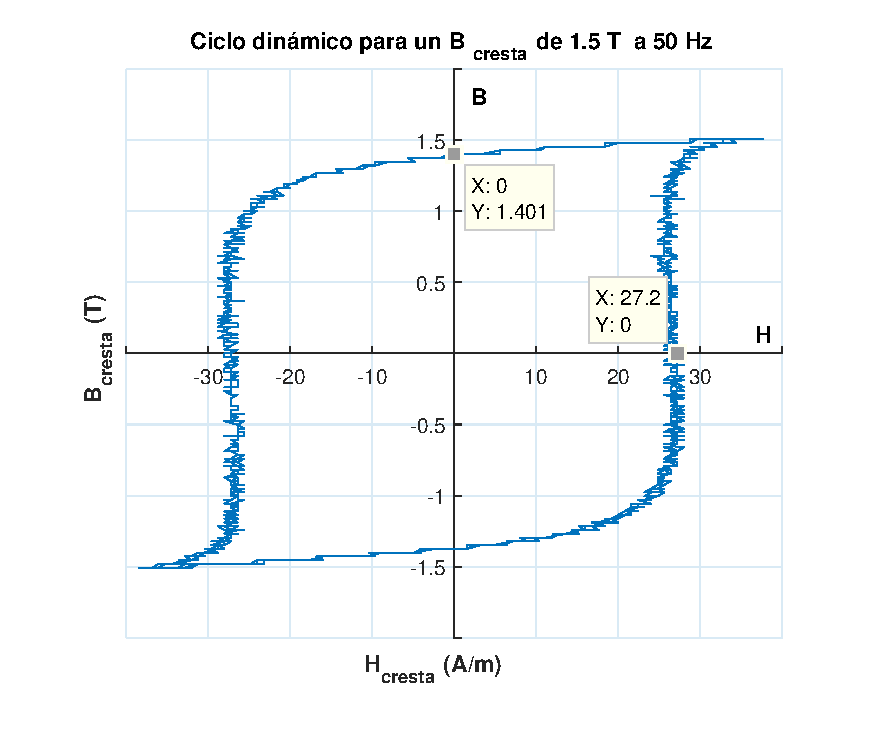
\includegraphics[width=\textwidth]{ciclo1.eps}
\end{figure}


\noindent\textbf{\underline{Resultados}}:
Los valores obtenidos de la inducción remanente y de la fuerza coercitiva son:
\begin{gather*}
    B_{remanente} = 1.401 \:T\\
    H_{f.coerct.} = 27.2\:A/m 
\end{gather*}
Incertidumbre de la medida de la inducción remanente:
\begin{gather*}
    \varepsilon(B_{rem})= \varepsilon(U_c^p)+\varepsilon(R_2)+\varepsilon(C) = 3\%+0.1\%+5\%=8.1\%
\end{gather*}
Incertidumbre de la medida de la fuerza coercitiva:
\begin{gather*}
    \varepsilon(H_{f.coerc.})= \varepsilon(R_1)+\varepsilon(U_{R_1}) = 0.1\%+2\%=2.1\%
\end{gather*}
Por lo que finalmente se tienen unas medidas de la inducción remanente de:
\begin{gather*}
    B_{rem}= 1.401\pm0.113\:T = 1.401\:T\pm 8.1\%
\end{gather*}
y una medida de la fuerza coercitiva de:
\begin{gather*}
    H_{f.coerct.} = 27.2\pm0.57\:A/m =27.2\:A/m\pm2.1\%
\end{gather*}
\noindent\textbf{\underline{Conclusiones}}:
La utilización de una resistencia de 100 m$\Omega$ empeora la representación del ciclo de dinámico \textit{B-H}, ya que se miden tensiones muy pequeñas en $R_1$ y el ruido, (que presenta un valor no despreciable respecto a la señal medida en el osciloscopio) impide la medida con buena precisión. Como se puede visualizar directamente en el \textit{display} del osciloscopio, con $U_{R_1}$ en el eje horizontal \textit{vs.} $U_{cond}$ en el eje vertical, se debe utilizar $R_1$=1 $\Omega$, para mejorar tanto la precisión como el ruido de la señal (150 mV frente a 15 mV).

\end{document}
